\begin{center}
\begin{tabular}{llrrrr}
\hline
Dataset & Search & Attr. & Cost & Inner Brier & Test Brier\\
\hline
Natural Scene & Full & 294 & 1648 & 0.259592 & 0.252943\\
Natural Scene & Joint & 5 & 6 & 0.258287 & 0.307503\\
Natural Scene & Pred. only & 5 & 9 & 0.250780 & 0.295259\\
Natural Scene & Guided & 6 & 12 & 0.259264 & 0.273556\\
SBU-3DFE & Full & 243 & 1373 & 0.027475 & 0.033553\\
SBU-3DFE & Joint & 11 & 14 & 0.027445 & 0.033364\\
SBU-3DFE & Pred. only & 4 & 14 & 0.026958 & 0.034414\\
SBU-3DFE & Guided & 5 & 20 & 0.027368 & 0.034423\\
Yeast-cold & Full & 24 & 127 & 0.007930 & 0.007210\\
Yeast-cold & Joint & 1 & 1 & 0.007213 & 0.007952\\
Yeast-cold & Pred. only & 0 & 0 & 0.006231 & 0.006442\\
Yeast-cold & Guided & 0 & 0 & 0.006231 & 0.006442\\
\hline
\end{tabular}
\end{center}
All three candidate outputs pass the fixed full-set prediction guard and
are single-deletion irreducible under that guard. The Natural Scene output
has dependency 0.102931, below its old floor 0.113918; it is valid under the
revised objective. Its test loss improves relative to both saved searches,
but its cost increases and its validation loss is closer to the allowed
limit. On SBU-3DFE, guidance increases cost and does not improve test loss
relative to either search. On Yeast-cold, the empty subset passes immediately,
so no dependency ranking is performed; its improvement over joint search
is due to removing the hard feasibility floor, not evidence of a benefit
from directed geometry. The development pilot therefore validates the new
predicate and permits lower-dependency solutions, but does not establish
a stable advantage of dependency-guided ranking. Further formal benchmark
expansion remains deferred.

\begin{figure}[htbp]
\centering
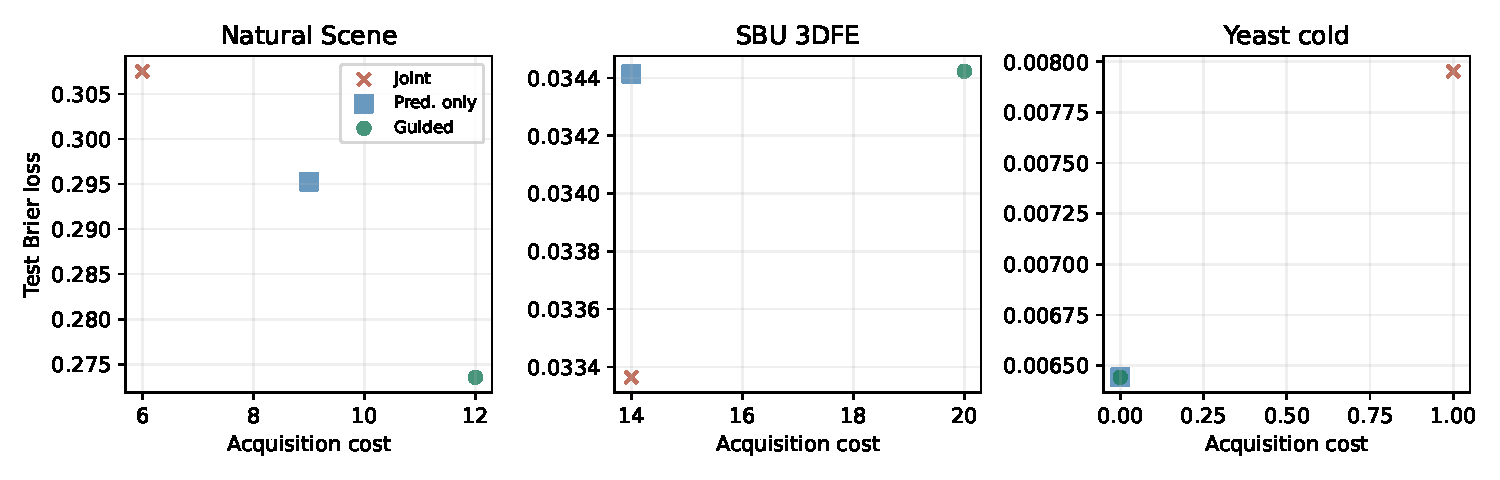
\includegraphics[width=\linewidth]{predictive_revision/pilot_comparison.pdf}
\caption{Development pilot on three previously examined splits. Points show
acquisition cost and saved test Brier loss for the two original searches
and the candidate guidance rule. Lower values are preferable on both axes.
The full-set losses are reported in the table; full-set costs lie outside
these reduced-search panels. Coincident Yeast-cold prediction-only and
guided points indicate the same zero-feature mean predictor.}
\end{figure}
